%----------------------------------------------------------------------------------------
%	PACKAGES AND OTHER DOCUMENT CONFIGURATIONS
%----------------------------------------------------------------------------------------

\documentclass[twoside]{article}

\usepackage{lipsum} % Package to generate dummy text throughout this template

\usepackage[sc]{mathpazo} % Use the Palatino font
\usepackage[T1]{fontenc} % Use 8-bit encoding that has 256 glyphs
\usepackage[utf8]{inputenc}
\linespread{1.05} % Line spacing - Palatino needs more space between lines
\usepackage{microtype} % Slightly tweak font spacing for aesthetics
\usepackage{graphicx}

\usepackage[hmarginratio=1:1,top=32mm,columnsep=20pt]{geometry} % Document margins
\usepackage{multicol} % Used for the two-column layout of the document
\usepackage[hang, small,labelfont=bf,up,textfont=it,up]{caption} % Custom captions under/above floats in tables or figures
\usepackage{booktabs} % Horizontal rules in tables
\usepackage{float} % Required for tables and figures in the multi-column environment - they need to be placed in specific locations with the [H] (e.g. \begin{table}[H])
\usepackage{hyperref} % For hyperlinks in the PDF

\usepackage{lettrine} % The lettrine is the first enlarged letter at the beginning of the text
\usepackage{paralist} % Used for the compactitem environment which makes bullet points with less space between them

\usepackage{abstract} % Allows abstract customization
\renewcommand{\abstractnamefont}{\normalfont\bfseries} % Set the "Abstract" text to bold
\renewcommand{\abstracttextfont}{\normalfont\small\itshape} % Set the abstract itself to small italic text

\usepackage{titlesec} % Allows customization of titles
\renewcommand\thesection{\Roman{section}} % Roman numerals for the sections
\renewcommand\thesubsection{\Roman{subsection}} % Roman numerals for subsections
\titleformat{\section}[block]{\large\scshape\centering}{\thesection.}{1em}{} % Change the look of the section titles
\titleformat{\subsection}[block]{\large}{\thesubsection.}{1em}{} % Change the look of the section titles

\usepackage{amsmath}
\usepackage{algpseudocode}
\usepackage{algorithm}

\newcommand{\todo}[1]{\textbf{TODO(#1)}}
\renewcommand{\v}[1]{\vec{#1}}

%----------------------------------------------------------------------------------------
%	TITLE SECTION
%----------------------------------------------------------------------------------------

% TODO: otsikosta saa 2/40 p, voi ansaita hiontaa kun työ on pidemmmällä. 

\title{\vspace{-15mm}\fontsize{24pt}{10pt}\selectfont\textbf{Predicting wine color and quality using chemical characteristics}}

\author{
\large
\textsc{A comparison of machine learning methods}\\[2mm]
\textsc{Hannu Siikonen, Mikko Perttunen}\\[2mm]
\vspace{-5mm}
}
\date{}

%----------------------------------------------------------------------------------------

\begin{document}

\maketitle % Insert title

%----------------------------------------------------------------------------------------
%	ABSTRACT
%----------------------------------------------------------------------------------------

\begin{abstract}
% TODO: myöskin 2/40 p, 100-200 sanaa

\noindent Katsoppas uudestaan. Utsoppas kaadestaan. Sas.

\end{abstract}

%----------------------------------------------------------------------------------------
%	ARTICLE CONTENTS
%----------------------------------------------------------------------------------------

\begin{multicols}{2} % Two-column layout throughout the main article text

\section{Introduction}
% 4/40 p
% Introduces the reader to the topic and the broad context within which the research fits
% Why is the task important, what question is being addressed, what is hoped to learn?
% Literature review

The goal of this study is to predict the type and the quality of a wine by making use of a given dataset.
This is realized by comparing the strengths and weaknesses of different machine learning 
and statistical modelling algorithms when applied to the present data. Optimized learning algorithms
are then revised based on the performance of different methods.
 
All possible algorithms cannot be well-equipped for these analyses. Nevertheless,
a variety of methods is used. This is important when dealing with a randomly chosen dataset, since according to
Wolpert\todo{\LaTeX-viittaus}, there is no simple way to predetermine which
learning algorithm yields the best results with the data. In other words, it can be difficult to assess
which method the inductive bias that corresponds best to the data without resorting to trial and error.
The evaluated algorithms were selected based on their diversity and using some initial hypotheses.

For the sake of variety, the performance of both regression and classification algorithms is evaluated.
However, the focus is on classification algorithms - to some extent due to it being more straightforward to compare the 
performance of classification models. Moreover, both the prediction of the type and the quality of the wine can be considered
classification problems, whereas only the quality can be studied also using regression. It is obvious that
there is some correlation between neighboring classes, that is, between wine quality values that differ by only one point. This makes
using regression a good idea, although on the other hand the integer presentation of the quality makes using regression somewhat cumbersome.

The dataset that is used to evaluate algorithms is derived from the so called \emph{Vinho verde} dataset by Cortez et al. \cite{CorCer09}.
It consists of 6000 observations, each describing an individual wine. For each one of them, 11 variables are provided in addition
to the color and quality of the wine: fixed acidity, volatile acidity, density, pH and amounts of citric acid, residual sugar, chlorides, 
free sulfur diodixe, total sulfur dioxide, sulphates and alcohol in the wine. The color of each wine is either red or white 
and the quality is an integer between 1 and 7. 5000 observations are used as training data, while the other 1000 are reserved for testing.

Wine data is in general a favored object for study in the field of machine learning. There have been various studies
on the subject, for instance those of Cortez et al. \cite{WQA}, \cite{CorCer09} 
and Appalsamy et al. \cite{Appalsami}. One motive for this are the large and growing markets of the wine industry.
Being able to predict the quality of a wine without the need for a wine taster, as well as a deeper understanding
of the properties of a good wine, induce much potential for profit. On the other hand, the problem of predicting
the quality of a wine is intriguing from a machine learning perspective. The quality is determined by human taste,
a very complex and subjective system, difficult to predict only by using a limited set of chemical properties.
One more reason to explain the popularity of wine quality predictions is the fact that there is a lot of data
on wines available on the Internet.

This task is interesting, since the prediction problem is twofold: both a clear physical property and an abstract, subjective property
are to be predicted. The former should be relatively easily predictable, assuming that a sufficient set
of chemical properties is given. The prediction of the quality, on the other hand, can be a very challenging task.
In general, these kinds of hard problems are often ones that are good for benchmarking machine learning algorithms.
In addition to that, with such difficult problems a great interest exists for a decently performant prediction algorithm,
since prioer to sufficient computing power and analysis methods they have been insolvable. Thus, this study provides a
good review of the features of modern machine learning algorithms when applied to a complex dataset.
 
\section{Methods}
% 8/40 p
% Methods used to conduct your experiment
% Concept-level: Methods/algos and modifications to these

For predicting the behavior of the wine data, many machine learning methods are equipped.
To some extent the same classification algorithms are used with minor differences for both
the analysis of the type and the analysis of the quality of wines. On top of this, to augur the 
quality, some regression algorithms are utilized. The basic properties of the used algorithms
are described in this section. The theoretical background of most of the algorithms can be found
in a basic reference, such as Ref. \cite{Alpaydin}. 

\subsection{Classification}

\subsubsection{Naive Gaussian discrimination} \label{method:naiivig}

While taking initial steps with a dataset, it is usually instructive to begin with a simple
learning algorithm. At the simplest, this could mean using a model that returns a constant value or
class. A slightly more complicated simple model is provided byt using only one of the eleven variables
given in the data. The initial hypothesis is that for some of the parameters, all classes are somewhat
normally distributed for this variable $x$. It follows that by calculating the mean value 
$\mu$ and variance $\sigma^2$ of each class using the training set, the probability distributions of 
each class $k$ is obtained:
\begin{equation}
 p(x|\mu_k,\sigma_k) = \frac{1}{\sqrt{2\pi} \sigma_k} e^{-\frac{(x-\mu_k)^2}{2\sigma_k^2}}.
\end{equation}
This can be used directly as a likelihood function for the different classes or a Bayesian posterior
can be taken:
\begin{equation}\label{posterior}
 p(\mu_k,\sigma_k|x) \propto p(x|\mu_k,\sigma_k) p(\mu_k,\sigma_k),
\end{equation}
where $p(\mu_k,\sigma_k) = p(\theta_k)$ is simply obtained as the fraction of the class $k$ in the 
training set. This can be transformed conveniently into a discriminant, by choosing a reference
class $j = k$:
\begin{equation}\label{naiividiskr}
 g_k(x) = \log \frac{p(\mu_k,\sigma_k|x)}{p(\mu_j,\sigma_j|x)}.
\end{equation}
The maximal $g_k(x)$ indicates the predicted class $k$. By simplifying Eq. \eqref{naiividiskr},
it is obtained
\begin{equation}\label{naiividiskr2}
 g_k(x) = \frac{(x-\mu_j)^2}{2\sigma_k^2}-\frac{(x-\mu_k)^2}{2\sigma_k^2} + 
 \log \frac{\sigma_j}{\sigma_k}.
\end{equation}


\subsubsection{Multivariate Gaussian discrimination}\label{method:multig}

The multivariate gaussian discriminant operates analogically to the one-dimensional
case, extending the discriminant function to eleven variables. It determines the class of a sample by
comparing the probabilities of it belonging to each class, when each
class is modelled using a multivariate Gaussian distribution. This can be problematic,
since many real-world variables have a clearly non-Gaussian distribution.

The Gaussian distributions are determined based on training data.
The mean vector $\v{\mu}_k$ and covariance matrix $\mathbf{\Sigma}_k$ are calculated for each class.
The probability of a sample $x$ belonging to the class can then be calculated
using the multivariate Gaussian probability density function:

\begin{equation}\label{monigauss}
 p(\v{x}|\v{\mu}_k,\mathbf{\Sigma_k}) = \frac{1}{\sqrt{2\pi} |\mathbf{\Sigma_k}|}
 e^{-\frac{1}{2}(\v{x}-\v{\mu}_k)^T \mathbf{\Sigma}_k^{-1} (\v{x}-\v{\mu}_k)}
\end{equation}

The likelihood of Eq. \eqref{monigauss} can be used directly for estimating the class of a
sample $\v{x}$, or a Bayesian posterior can be utilized as in Eq. \eqref{posterior}. 
A discriminant can be constructed parallelly to Eqs. \eqref{naiividiskr} and \eqref{naiividiskr2}:
\begin{equation}
	\begin{aligned}
	 g_k(\v{x}) = \frac{1}{2}(\v{x}-\v{\mu}_j)^T \mathbf{\Sigma}_j^{-1} (\v{x}-\v{\mu}_j) - \\
	 \frac{1}{2}(\v{x}-\v{\mu}_k)^T \mathbf{\Sigma}_k^{-1} (\v{x}-\v{\mu}_k) 
	+\log \frac{|\mathbf{\Sigma}_j|}{|\mathbf{\Sigma}_k|}.
       \end{aligned}
\end{equation}
Again, the class with the largest discriminant $g_k(\v{x})$ indicates the prediction of klass, $k$.

\subsubsection{$k$ nearest neighbours}\label{method:knn}

The $k$ nearest neighbours classifier is a non-parametric classifier. Only a
distance function between the points in the variable space is required.
The classification given by $k$ nearest neighbours for a new point $\v{x}$ is then found by simply
selecting the $k$ points closest to $x$ according to the distance function and
picking the most common class among the $k$ points. The training set is fully
stored in memory. The samples in it are used for the nearest neighbour study
of the points in the validation or the test set.

Selecting a good distance function is important, especially when many variables
are used for the prediction. The distributions of the
input variables can vary greatly. When using the Euclidean distance function,
this causes certain variables to have a greater effect on the distance between
points when compared to others. To prevent this, we used the Mahalanobis
distance function\cite[p.~88]{Alpaydin}:

\begin{equation}\label{eq:mahalanobis}
  D_M(\v{x}, \v{y}) = \sqrt{(\v{x}-\v{y})^T \Sigma^{-1} (\v{x}-\v{y})}
\end{equation}

where $\Sigma$ is the covariance matrix for the 
distribution $\v{x}$ and $\v{y}$ are taken from.
This normalizes the distances in the different dimensions of
the variable space and also takes into account unneccessary correlations.
The Mahalanobis distance is an intuitive distance measure for an arbitrarily
scaled space. It appears for instance in the exponent of the multivariate
Gaussian distribution of Eq. \eqref{monigauss}.

If the class probabilities $p_c(\v{x})$ for a point $\v{x}$ are required, these can
be calculated using the nearest neighbours of it. If the frequency of a class $c$
within the $k$ nearest neighbours is $k_c$, the probability is simply
\begin{equation}
 p(\v{x}) = \frac{k_c}{k}.
\end{equation}

\subsubsection{Linear discrimination}\label{method:ldiskr}

The methods that rely on discrimination model directly the class discriminants instead of
the class probabilities. In linear discrimination the discriminant for a class $k$ is linear:
\begin{equation}
 g_k(\v{x}) = \v{w}_k^T v{x} + w_{k0}.
\end{equation}
The basic theory of linear discrimination is not deeper than this: the goal is to find such
coefficients $\v{w}_k$, $w_{k0}$ that the classification error is minimal. Usually this has
to be done numerically for instance with the steepest descent algorithm. There are multiple 
ways to perform the optimization. One example
is logistic discrimination, in which the class probabilities are defined by a connection to the class
probabilities. The discriminant of a class $k$ is a logarithm of the fraction of the likelihood of
this class divided by the likelihood of a reference class. This definition gives some convenient 
properties for the model from the viewpoint of numerical solutions. However, also other
approaches may be used.

\subsubsection{Quadratic discrimination}\label{method:qdiskr}

Quadratic discrimination is otherwise similar to linear discrimination, but it equips a quadratic discriminant,
\begin{equation}
 g_k(\v{x}) = \v{x}^T \mathbf{W}_k \v{x} + \v{w}_k^T \v{x} + w_{k0}.
\end{equation}
Because of the quadratic form, the search for optimal discriminants is much more complicated than with linear
discriminants. Additionally, the additional complexity brought by the quadratic form may be unnecessary.
Nevertheless, quadratic discrimination provides a good algorithm for comparison, if an efficient algorithm
for it is available.

\subsubsection{Support vector machine}\label{method:svm}

Support vector machines are a variant of linear discrimination. If classes do not overlap, it finds
the separating hyperplanes between classes that have the largest margins. These hyperplanes correspond 
to the linear discriminants. With overlapping classes, a penalty term is added to the solution in order
to make the same approach work. The discriminants trained with the training set are used for validation
and test sets.

\subsubsection{Random forest}\label{method:randfor}

Random forest \cite{Forest} is an ensemble learning method that equips an ensemble of classification trees. Each tree 
in the ensemble does classification using only a chosen number of the given variables. This could be for
instance the square root of the total amount of variables. For this kind of an ensemble of trees
the trees themselves are usually unpruned. The trees themselves are simply ordinary classification trees:
they use the given variables and split the branches until a desired amount of purity or other conditions
are fulfilled for the training set. It is utterly important that there is a sufficient amount of classification
trees in the ensemble. With a too small amount of trees sufficient statistics are not reached and the algorithm
does not perform optimally.

\subsection{Regression}

\subsubsection{Random forest, regression}

The random forest algorithm can be used also for regression. In this case, the classification trees in the 
ensemble are substituted with regression trees. A regression tree gives effectively a constant value as an output,
since a typical tree cannot easily give continuous output. When an ensemble of regression trees is considered, the 
situation is a bit more interesting. The final output is averaged over many trees and thus the output resembles
more a continuous behaviour.

\subsubsection{Linear least squares}\label{method:leastsquare}

The linear (or ordinary) least squares method is a regression algorithm that
finds a linear fit for one variable as a function of multiple variables: $\hat{y} = \v{a}^T \v{x}+b$. 
The vector $\v{a}$ and the constant $b$ are such that in the training set $\sum (y - \hat{y})$ is 
minimized, hence the name least squares.

The problem can be conveniently presented in a matrix form. Let $\mathbf{X}$ be a matrix
with rows $[1, \v{x}^T]$, composed of all the samples in the training set. That is, the 
constant $b$ is now included in the vector for the sake of convenience. Let $\v{y}$ be
a corresponding column vector and $\v{w}$ a column vector that holds the linear coefficients and
\begin{equation}
\hat{\v{y}} = \mathbf{X} \v{w}
\end{equation}
is the least squares estimate. Now the least squares problem is equal to minimizing the
vector product $(\v{y} - \hat{\v{y}})^T(\v{y} - \hat{\v{y}})$ with respect to $\v{w}$. 

It can be briefly shown that the optimal solution is given by 
\begin{equation}
 \v{w} = (\mathbf{X}^T \mathbf{X})^{-1} \mathbf{X}^T y.
\end{equation}
This is a usuful form, since it can be used for an arbitrary matrix $\mathbf{X}$. That is,
$\mathbf{X}$ may hold only the given variables in a basic form, but also for instance higher
exponents of the variables can be inserted into this matrix. Thus, it is relatively simple
to control the complexity of this model.

\subsection{PCA}\label{method:pca}

Primary Component Analysis is a useful method that can be used with both classification and regression
problems. Effectively, it reduces the amount of variables that the variable that is predicted depends
on. This can be useful, if some of the provided data is not at all useful in the analysis. On the other
hand, it gives an effective method of graphical representation of the data. If the studied variable
depends on over three dimensions, using PCA it can be projected to three or two dimensions. This is
helpful while trying to develop a concrete understanding of the data used.

PCA itself relies on studying the parameters that are responsible for most of the variance of the studied
variable. The greater the effect on variance, the more the parameter explains the behaviour of the variable.
Mathematically, PCA studies the covariance matrix of the matrix that holds the training set samples of the 
variables that are used to predict the variable of interest. The eigenvectors of the covariance matrix are
the principal components. The corresponding eigenvalues indicate the relative fraction of variance that
the principal components (eigenvectors) are responsible for. 

If PCA is done with a reduction from $N$ to
$K$ dimensions, the $K$ largest eigenvalues of the covariance matrix are chosen. The data in the training set is shifted so that
its mean value is zero in all dimensions, and then it is projected on the $K$ eigenvectors that correspond
to the chosen eigenvalues. This is the PCA-representation, which can be used for graphical purposes or
also as the input data for machine learning algorithms.

\subsection{Combining learners}\label{method:combo}

If many different learners with approximately equal performance are found, it is instructive
to combine these learners to boost performance. For this, many kinds of algorithms can be used
but in this work a simple approach is taken. It is assumed that maximally three very good
learning algorithms are chosen for the final model. With these algorithms, the probabilities
of each class are calculated for each sample in the validation or testing set. The probabilities
are denoted with $P_1$, $P_2$ and $P_3$ and they are given weights $w_1$, $w_2$ and $w_3$.
The weights are normalized so that $w_1 + w_2 + w_3 = 1$. Thus the final probability is given by
\begin{equation}
 P = w_1 ( P_1 - P_3 ) + w_2 ( P_2 - P_3 ) + P_3.
\end{equation}
Because of the normalization condition and assumption that the weights are greater than zero,  $0 \leq w_1,w_2 \leq$ and $w_1 + w_2 \leq 1$. 
An approximate solution can be found by scanning the possible values of $w_1$ and $w_2$ on a lattice with a spacing of $0.01$.
The best values are chosen by validation. In this work the goal is that no more than three learning algorithms are combined.
With only two learning algorithms, only one parameter has to be scanned over.

%\begin{figure}[H]
%\centering
%\includegraphics[width=0.5\textwidth]{learning}
%\caption{Learning is important but big processors are importanter. \cite{alpaydin2004introduction}}
%\label{fig:learning}
%\end{figure}

%------------------------------------------------

\section{Experiments}
% 8/40 p
% Method and materials (applied)
% Necessary for applying the methods to the data: pre-proc., validation of params (cross-validation)
% No results here!

The study is divided into two different problems: the prediction of the type (color) and the quality (ranking)
of wines. Of these the latter is a considerably more demanding task, since the quality consists of more classes than the type and the
ruling mechanism of the human taste is complicated. To probe the data, at first simple algorithms are used for 
both the tasks, after which more complicated methods are used. This is a good way of keeping the analysis reasonable as
the hypothetically inferior algorithms give a starting level for the required performance. If a hypothetically
well-perporming algorithm performs actually similarly as a naive algorithm, it can be rejected.

For the actual analysis, matlab is used for the most part. It would be possible to implement these algorithms by hand,
but it makes more sense to use the algortihms that are already supplied by matlab. This way, it is possible to focus
on the actual properties of the algorithms, and not on optimizing each type of algorithm. The latter option could be
unrewarding, since all algortihms do not perform well, when some initially random data is studied.

\subsection{Method validation}

Method validation is done using $k$-fold cross validation with $k = 10$. That is, the training set is partitioned in 10 equally sized parts. 
Validation is done ten times using each partition once as a validation set, while the other nine
sections function as training sets. The mean error of the 10 different validations is used as a measure
of goodness of an algorithm. This is beneficial for choosing between different algorithms or
between parameter values with a single algorithm.

Cross-validation can be a bit problematic if it is used both for choosing parameter values for a single algorithm (e.g., the value of $k$
for the kNN-algorithm) and evaluating the goodness of the method. In such a case the choice of the parameter value makes the estimator
of goodness somewhat biased, which is harmful when making decisions between the algorithms. However, with the given amount of data
the 10-fold cross-validation is in general a good choice. Since $9/10$ of the whole training data is used as a training set at a time,
the situation resembles very much that of the actual final training phase. While training the final learning algorithm, the whole training dataset
is used. On the other hand, the small size of a single validation set is averaged out by considering all 10 different validation sets.
It is regrettable that in the validation the training sets have a large overlap. Nonetheless, it is not easy to use a given amount
of training data more economically than with $k$-fold cross-validation.

\subsection{Algorithm evaluation}

While using learning algorithms, type is not used as a predictor for quality nor quality for color.
In principle, such a measure could be useful. If either quality or color was predicted very
accurately, there would be new information in the decision process of determining the classes of these.
However, there is a great amount of uncertainty involved in using an already predicted value as a
parameter of a second learner. If a test set differs significantly from the training set, this could
make the second algorithm perform poorly.

Some of the algorithms are used for the study of both problems while others are only applied to one of them.
Knowledge of chemistry or any other kind of preliminary knowledge of wines is not used. The problems are treated purely as machine learning
problems. The greatest external utility in this context is the set of the variables that are used for the predictions.
These were supplied in beforehand and it can be assumed that they are useful in the problems. PCA and similar methods are useful
for studying, whether there is some useless variables in the given dataset. On the other hand, the final testing results imply, whether the supplied
data was sufficient.

For evaluating the performance of different algorithms a couple of different methods are used. The 
most basic measure is the total amount of false augurs, when the problem is treated as classification.
This gives a general view of the situation, but does not give a complete picture of the situation. For instance
with classification problems one can predict that all the samples in the test data belong to one class. If
this class has a high prior probability, it can be supposed that a large amount of predictions are correct.
This is, however, problematic, since only the members of one class are predicted correctly. A simple algorithm
could give a similar error rate as the given naive assumption, but it would probably also have a non-zero success
rate for the other classes. This is preferable and, therefore, a more complicated measure of goodness, \emph{f-score}, is used:
\begin{equation}
 \text{f-score} = \frac{ 2 \cdot \text{precision} \cdot \text{recall} }{\text{precision} + \text{recall}}.
\end{equation}
This measure is used for each class within the study. To get the total f-score of a prediction, a weighted sum of
the f-scores of the classes is taken. The weights are normalized and proportional to the amount of samples in
each class in the set that is being predicted. Here the following definitions are used:
\begin{eqnarray}
 &\text{precision} & = \frac{N_{tp}}{N_{tp}+N_{fp}} \\
 &\text{recall} & = \frac{N_{tp}}{N_{tp}+N_{fn}}.
\end{eqnarray}
The $N$ -quantities refer simply to the amounts of samples of certain types. The letter $t$ stands for true and $f$ for false.
Additionally $p$ stands for positive and $n$ for negative. By using this kind of a definition the evaluation of goodness
is more complicated than a simple fraction of errors. The more correct predictions one class receives, the less it raises
the total f-score of an algorithm. On the other hand, a class with only a few correct predictions benefits much more from
a raise in the amount of true positives. Thus, using f-score, more value is given for the \emph{variety of classes}.

Since the prediction of quality has some regressive nature, an additional score more fitting for regression was given
for the forecasts of quality. The score is defined as a mean squared error:
\begin{equation}
 \epsilon = \frac{1}{N} \sqrt{ \sum_{i=1}^N ( \text{prediction}_i - \text{true}_i )^2 }.
\end{equation}
This score indicates how much the predicted quality differs from the actual quality. This score type is more of a curiosity,
but it helps in obtaining a full picture of the situation.

\subsection{Prediction of type}

In principle the prediction of type should be a task that is easily regressed to the chemical properties of a wine.
The most significant distinction between white and red wines is the color, which has its foundation in the fine structure of 
the wine. Still, there is not much knowledge of the type at beforehand and thus different methods are tested.

\subsubsection{Simple classification methods}

The analysis of algorithms is initiated with simple algorithms. The first prediction that is made is simply a constant
type. Since there are only two types available, this will by definition give an error rate that is below $50\%$. However,
at least the f-score should be relatively low, except for if there are few wines of the second type available. With the given
data it will turn out that the more frequent wine type are the white wines, but this is not yet relevant.

As a first real algorithm we use the naive Gaussian estimate as described in section \ref{method:naiivig}. With this it is
important to find a variable for which the types are even somewhat distributed in the shape of a bell curve. The obtained 
result is a numerically unchallenging and simple prediction. From this the analysis can be logically widened to a full
multivariate Gaussian prediction, as shown in section \ref{method:multig}. This should work better than a univariate
Gaussian method even if the variables were not in general distributed in a Gaussian way. If there is at least some
clustered behaviour of classes as a function of some variables, the approach is helpful. For both the multivariate
and univariate Gaussian cases also Bayesian prior probabilities are applied. This way, the performance should be 
slightly boosted.

Thus, three initial methods are developed. None of these are actually expected to perform very well, since the inductive
biases are obviously significant. However, now a solid basis is set for further analyses.

\subsubsection{More involved classification methods}

Some methods are used for the classification scheme. There is actually no good initial knowledge on what kind of a classifier
would perform well in the given situation. Therefore, the algorithms have to be simply tested out. Here, some preliminary 
pruning has been performed in order to obtain a remarkably diverse set of algorithms.

The linear discriminant method is used to make a somewhat generic prediction for the classification. This divides the variable space
with hyperplanes, which separate each class to a confined area. While the algorithms of matlab are used, also a quadratic discriminant
could be in principle equipped. In general, this is not that advisable because the full quadratic form adds much unneccessary complexity
to the model. This way, the model is likely to be fitted unoptimally to the given data. Therefore, only a simple linear discrimination is used.

To contribute to the results of a linear discriminant, also a $k$ Nearest Neighbours -model is used. In this case it is important to choose
a fitting value for the parameter $k$. The 10-fold cross-validation method is fitting for this choise. It should be noted that if the model
tends to be optimal with small values of $k$, its probability-related features are diminished. As an extreme, with $k=1$ the class probabilities
of a point in the test set are 0 or 100 $\%$. Probability-related properties are important while models are combined and thus also this aspect
should be taken into account.

As a last choice the Random Forest algorithm is used. It combines both ensemble methods and classification trees. For this algorithm both the size
of the forest and the amount of parameters used for classification has to be chosen. The size of the forest means the amount of trees in the ensemble.
Making this parameter larger is good for the results but it will increase the calculation time. For the amount of variables used in a single tree a
value clearly smaller that 11 should be used. This mean approximately 4 or less variables. In general, less variables can be good so that
all variables are taken properly into account. On the other hand, less variables in a tree means a demand for using a larger forest. Thus,
with this algorithm matters related to computational time become important.

\subsubsection{PCA}

Primary component analysis can be useful in pre-processing data, at least if some \emph{unnecessary} data is given. Thus, it is good to check, whether
using it is beneficial with the current data. It can also depend on algortihm, whether or not PCA gives enhanced results. The $k$NN-algorithm and random
forest in general are friendly with a high dimensionality. Thus, a reduction in dimensionality may not be very helpful. On the contrary, the linear discriminant
method may obtain significant advantage of having to use less dimensions. Thus, this method is tested with different amounts of projection dimensions.

\subsubsection{Combining algorithms}

If the performance of multiple algorithms is in the same scale, these algorithms should be combined to obtain even better results. It depends on the amount
of methods to be combined, how complex this process is. However, maximally 3 methods are combined and this can be done in the way described in section \ref{method:combo}.

\subsection{Prediction of Quality}

There are various possible problems that can arise in the prediction of the quality. One initial issue is that it is
not known, whether it is more favorable to use classification or regression algorithms. This has to be also tested
to some extent, to have a good picture of the two different approaches. Otherwise there are much similarities to the 
prediction of type with the distinction that many aspects are now a bit more complicated. There are more classes, which
makes things more difficult in many ways.

\subsubsection{Classification}

Various algorithms for classification is used for the prediction of quality. Also in this case linear discrimination is used, as well 
as the support vector machine and a quadratic discrimination. This is mostly ruled by the complexity of the problem. It is instructive
to probe different discrimination methods, to determine if they are useful in the current problem. The quadratic discriminant could
actually be helpful in this case because of the hypothetic complexity of the problem.

For a basic classifier there is again a \emph{constant class} classifier but this time no Gaussian classifiers are used. This decision
is affected by the fact that the Gaussian nature of the data is not strong. Additionally, for seven classes this type of classification
is not easily performed. Univariate classification can be directly left out, since there is much room for problematic behaviour when
many classes are fitted into one dimension. On the other hand the full mutlivariate case is cumbersome to use and is not worth the 
additional effort, since other algorithms are probably better.

Additionally, also the $k$ Nearest Neighbors and random forest classification are used once again. In principle, there are only minor
differences when compared to the use of these algorithms in the case of type prediction.

\subsubsection{Regression}

For comparison, regression algorithms are used. There are two relevant questions: how does a regression algorithm perform in the context
of regression and how does it perform in the context of classification. For the context of regression, the additional score type was
given. If a regression algorithm seems to perform well, assessed in one way or another, it may be used for the final model.

The random forest algorithm is powerful and convenient to use and it can be applied also for regression. Its usage is simple,
since the only difference to classification is that the final result is not an integer. The result is rounded to the nearest
integer, to make it compatible with the \emph{real} results.

In addition, the least squares method is utilized, as shown in \ref{method:leastsquare}. This is somewhat compulsory, taking
into account that the least squares method is very popular in regression application. This algorithm can be conveniently
handled with matrix calculations.

\subsubsection{PCA and Combining algorithms}

With the experience gained from type prediction it is determined, whether it is useful to try PCA 
in this context. On the other hand, algorithm combination has the same rules as in the case of 
type. If there are algorithms that have a somewhat similar performance level, they should be
combined. If one algorithm is clearly better than the others, it can be used alone for the final predictions.

% \begin{table}[H]
% \caption{My current knowledge of tables}
% \centering
% \begin{tabular}{cc}
% \textbf{Table type} & \textbf{Likely location}\\
% \midrule
% Coffee table & Living room\\
% Dining table & Dining room\\
% Bedside table & Bedroom
% \end{tabular}
% \end{table}

%------------------------------------------------

\section{Results}
% 4/80 p
% Description of results with figures and tables

The analyses of algorithmical performance was carried out so that the color was analyzed first and then the quality. The final learning algorithm
was chosen by optimization among the used algorithms. Thus, there had to be some \emph{communication} between obtaining results and enhancing the models.

\subsection{Prediction of type}

The performance of multiple algorithms was tested using cross validation on the training dataset and for comparison also the performance in the testing data was studied.
F-score and total error rate were calculated for the naive Gaussian discriminant, multivariate Gaussian discriminant, linear discrimination, $k$ Nearest Neighbors and random forest
algorithms, as well as for the final hybrid algorithm.
Since a majority of the test observations consists of white wines, an intuitive dummy model predicts that all wines are white. The performance of this dummy model
is also included in the results.
For each evaluated algorithm, the rate of successful predictions and the F-score are reported. In addition, the success of the predictions are shown on PCA projections
of the observations. These are given in appendix \ref{appendix:colorpcakuvet}.

The training and testing datasets can be visualized by projecting into a two-dimensional plane using principal component analysis. By taking a look at
figures~\ref{fig:color_training_pca} and~\ref{fig:color_testing_pca} we can see that while the data is somewhat separated into groups by PCA,
the separation is not complete. In the figures blue dots are used for marking the white wines and red dots for marking the red wines.

\begin{figure}[H]
\centering
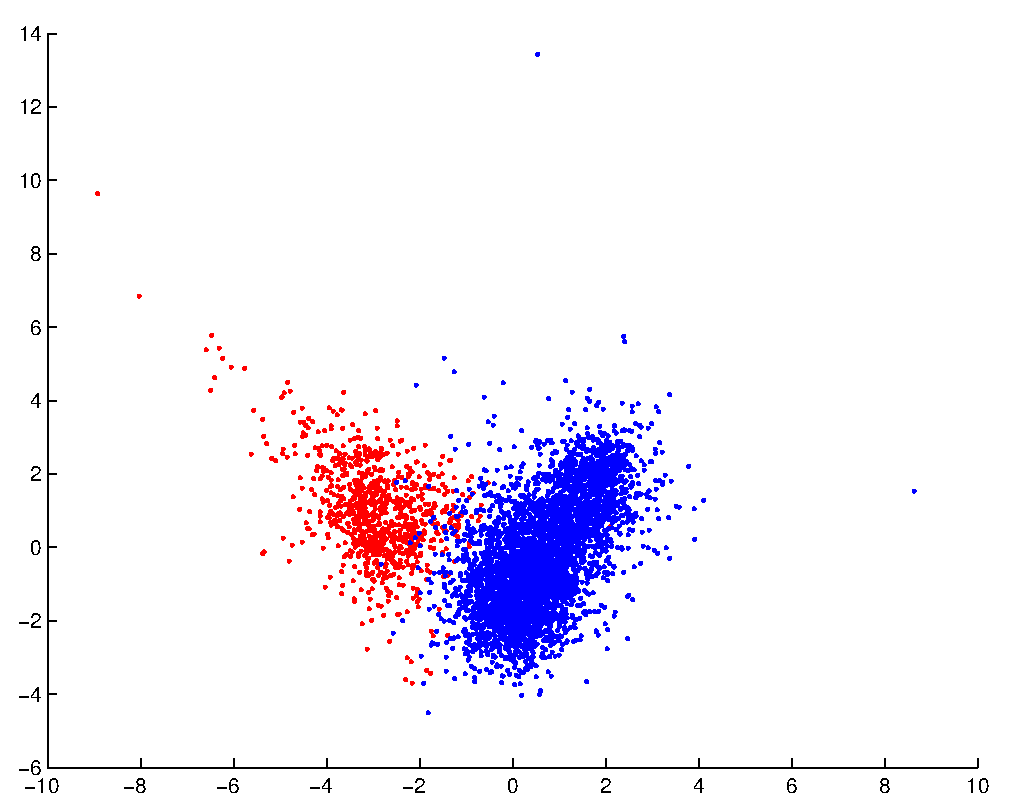
\includegraphics[width=0.5\textwidth]{trainingpca}
\caption{PCA projection of training dataset}
\label{fig:color_training_pca}
\end{figure}

\begin{figure}[H]
\centering
\includegraphics[width=0.5\textwidth]{testpca}
\caption{PCA projection of testing dataset}
\label{fig:color_testing_pca}
\end{figure}

\subsubsection{$k$NN cross-validation}

\subsubsection{Random forest cross-validation}

\subsubsection{Cross-validation between algorithms}

To determine, which algorithms should be used for the final evaluation a 10-fold cross-validation was performed. As a result, error values and f-scores were obtained.
These are useful for estimating the actual performance of the algorithms in a test set. 

Table~\ref{table:color_validation} shows the mean error rates and f-scores for each evaluated algorithm obtained in validation. The values are averaged over each
cross-validation partition on the training data.

\begin{table}[H]
\caption{Color prediction - validation}
\label{table:color_validation}
\begin{tabular}{lll}
\textbf{Method} & \textbf{Error rate} & \textbf{F-score}\\
\midrule
Dummy & 18.12\% & 0.737 \\
\\
\multicolumn{3}{c}{\textbf{Naive Gaussian}} \\
Uniform prior & 27.44\% & 0.756 \\
Proportional prior & 22.90\% & 0.782 \\
\\
\multicolumn{3}{c}{\textbf{Multivariate Gaussian}} \\
Uniform prior & 2.22\% & 0.978 \\
Proportional prior & 1.94\% & 0.981 \\
\\
\multicolumn{3}{c}{\textbf{Other methods}} \\
Linear discrimination & 0.66\% & 0.993 \\
$3$ nearest neighbours & 0.75\% & 0.993 \\
Random forest & 0.50\% & 0.995 \\
Hybrid & 0.38\% & 0.996 \\

\end{tabular}
\end{table}

\subsubsection{Testing}

To study the true performance of the final model(s), f-scores and error rates were calculated also using the test set. To view
the goodness of the choice of algorithms by cross-validation, these were calculated for all the methods used. 
Table~\ref{table:color_testing} shows the error rates and f-scores for each algorithm studied.

\begin{table}[H]
\caption{Color prediction - testing}
\label{table:color_testing}
\begin{tabular}{ccc}
\textbf{Method} & \textbf{Error rate} & \textbf{F-score}\\
\midrule
Dummy & 19.60\% & 0.717 \\
\\
\multicolumn{3}{c}{\textbf{Naive Gaussian}} \\
Uniform prior & 30.00\% & 0.730 \\
Proportional prior & 25.60\% & 0.756 \\
\\
\multicolumn{3}{c}{\textbf{Multivariate Gaussian}} \\
Uniform prior & 2.30\% & 0.977 \\
Proportional prior & 1.90\% & 0.981 \\
\\
\multicolumn{3}{c}{\textbf{Other methods}} \\
Linear discrimination & 0.30\% & 0.997 \\
$3$ nearest neighbours & 0.50\% & 0.995 \\
Random forest & 0.30\% & 0.997 \\
Hybrid & 0.20\% & 0.998 \\

\end{tabular}
\end{table}

\subsection{Quality prediction}

The performance of the linear discriminant, quadratic discriminant, support vector machine, $k=1$ nearest neighbors and random forest
classification algorithms, as well as the random forest and linear least squares regression algorithms were tested using cross validation 
on the training dataset and a testing dataset.
Since the majority of the test observations are of quality 4, a natural dummy model is to assume that all wines have quality 4.
This dummy model is also included in the results.
For each evaluated algorithm, the classification error rate, the F-score, and mean real distance are reported. In addition, the predictions are shown on a PCA projection
of the observations. These projections can be found in appendix A.

The training and testing datasets can be visualized by projecting into a two-dimensional plane using principal component analysis. Looking at
figures~\ref{fig:quality_training_pca} and~\ref{fig:quality_testing_pca} we can see that contrary to the color visualization, there are no clear groups
formed by different wine qualities.

\begin{figure}[H]
\centering
\includegraphics[width=0.5\textwidth]{qpcatraining}
\caption{PCA projection of training dataset. Blue is bad, red is good quality.}
\label{fig:quality_training_pca}
\end{figure}

\begin{figure}[H]
\centering
\includegraphics[width=0.5\textwidth]{qpcatesting}
\caption{PCA projection of testing dataset. Blue is bad, red is good quality.}
\label{fig:quality_testing_pca}
\end{figure}

\subsubsection{Validation}

Table~\ref{table:quality_validation} shows the mean error rates, f-scores, and mean real distances for each evaluated algorithm when run against the validation data. The values are averaged across each
cross-validation partition on the training data.

\begin{table}[H]
\caption{Quality prediction - validation}
\label{table:quality_validation}
\centering
\begin{tabular}{cccc}
\multicolumn{3}{l}{\textbf{Method}} \\
\textbf{Error rate} & \textbf{F-score} & \textbf{Distance} \\
\midrule
\multicolumn{3}{l}{Dummy} \\
56.06\% & 0.2685 & 0.0398 \\
\multicolumn{3}{l}{Linear discriminant} \\
46.14\% & 0.5111 & 0.0360 \\
\multicolumn{3}{l}{Quadratic discriminant} \\
51.80\% & 0.4787 & 0.0391 \\
\multicolumn{3}{l}{Support vector machine} \\
46.96\% & 0.4576 & 0.0368 \\
\multicolumn{3}{l}{$1$ nearest neighbor} \\
41.74\% & 0.5810 & 0.0377 \\
\multicolumn{3}{l}{Random forest} \\
35.06\% & 0.6293 & 0.0311 \\
\multicolumn{3}{l}{Random forest (regression)} \\
39.62\% & 0.5742 & 0.0320 \\
\multicolumn{3}{l}{Linear least squares} \\
47.24\% & 0.4907 & 0.0362 \\
\end{tabular}
\end{table}

\subsubsection{Testing}

Table~\ref{table:quality_testing} shows the mean error rates, f-scores, and mean real distances for each evaluated algorithm when run against the testing data.

\begin{table}[H]
\caption{Quality prediction - testing}
\label{table:quality_testing}
\centering
\begin{tabular}{cccc}
\multicolumn{3}{l}{\textbf{Method}} \\
\textbf{Error rate} & \textbf{F-score} & \textbf{Distance} \\
\midrule
\multicolumn{3}{l}{Dummy} \\
59.20\% & 0.2356 & 0.0286 \\
\multicolumn{3}{l}{Linear discriminant} \\
47.70\% & 0.4945 & 0.0249 \\
\multicolumn{3}{l}{Quadratic discriminant} \\
53.70\% & 0.4541 & 0.0279 \\
\multicolumn{3}{l}{Support vector machine} \\
50.10\% & 0.4279 & 0.0264 \\
\multicolumn{3}{l}{$1$ nearest neighbor} \\
41.90\% & 0.5789 & 0.0259 \\
\multicolumn{3}{l}{Random forest} \\
35.60\% & 0.6285 & 0.0216 \\
\multicolumn{3}{l}{Random forest (regression)} \\
39.50\% & 0.5757 & 0.0226 \\
\multicolumn{3}{l}{Linear least squares} \\
48.80\% & 0.4740 & 0.0249 \\
\end{tabular}
\end{table}

%------------------------------------------------

\section{Discussion}
% 4/80 p

Pohdinnot, results:issa vain raportointi, ei pohdintaa.

%----------------------------------------------------------------------------------------
%	REFERENCE LIST
%----------------------------------------------------------------------------------------

% 2/80 p
\bibliographystyle{plain}
\bibliography{final_report}{}

%------------------------------------------------
\appendix

\section{PCA type prediction}\label{appendix:colorpcakuvet}
% 4/80 p
% koodi-otteita
PCA projections that show, which predictions have failed for each algorithm.

%----------------------------------------------------------------------------------------

\end{multicols}

\end{document}
